\chapter{Indledning}
Aalborg Kommune er med et indbyggertal på over 200.000 og et areal på cirka  $1,\!140 km^2$ en af landets største kommuner \citep{kommunedata}. Det område, som Kommunen dækker, er vist på Figur \ref{fig:aalborgkommune}. 

\begin{figure}[htbp]
	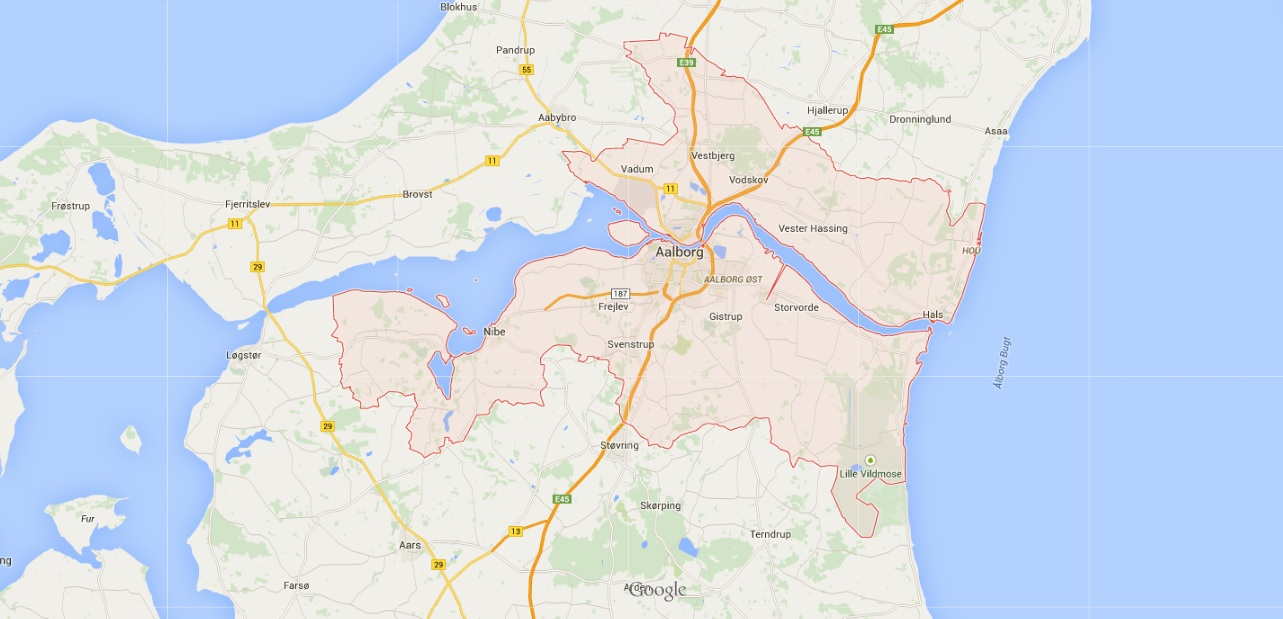
\includegraphics[width=1.0\textwidth]{billeder/aalborgkommune.png}
	\caption{Aalborg Kommune}
	\label{fig:aalborgkommune}
\end{figure}

\indent{     }  Aalborg er en tidligere industriby, og førhen var industriområderne placeret i Aalborg Centrum. Nye planer for Aalborg har ført denne industri ud i nogle yderpunkter af Aalborg by. Derfor har kommunen nye visioner om at flytte kultur, studieliv og turisme ind, hvor der før var industri. Kommunens visioner omkring byens udvikling fremgår af Kommuneplanen, hvor det primære fokus i denne rapport vil være et område gennem Aalborg, der er tiltænkt meget vækst; dette betegnes som Vækstaksen (se Figur \ref{fig:vaekstakse}).
\newline \indent{     }  Indenfor de seneste 10 år har Aalborgs havnefront gennemgået en stor udvikling. Denne er stadig i gang, hvilket ses ved, at der kommer flere boligbyggerier til havnen, som Strøybergs Palæ er en del af. 
\newline \indent{     }  Det har siden år 2010 været på tale, at lave en tilbygning til den bevaringsværdige bygning Strøybergs Palæ. Hovedbygningen af Strøybergs Palæ er fra år 1900 \citep{hovedbygning}, mens sidebygningen er fra år 1908 \citep{sidebygning}, beliggende centralt i Aalborg ved Slotspladsen, der er en cirka 200 m vejstrækning og plads ved Aalborgs centrale havnefront, samt i nærheden af museet Utzon Centret og overfor shoppingcentret Friis. Figur \ref{fig:aalborg} viser Strøybergs Palæs beliggenhed i Aalborg. 

\begin{figure}[htbp]
	\centering
	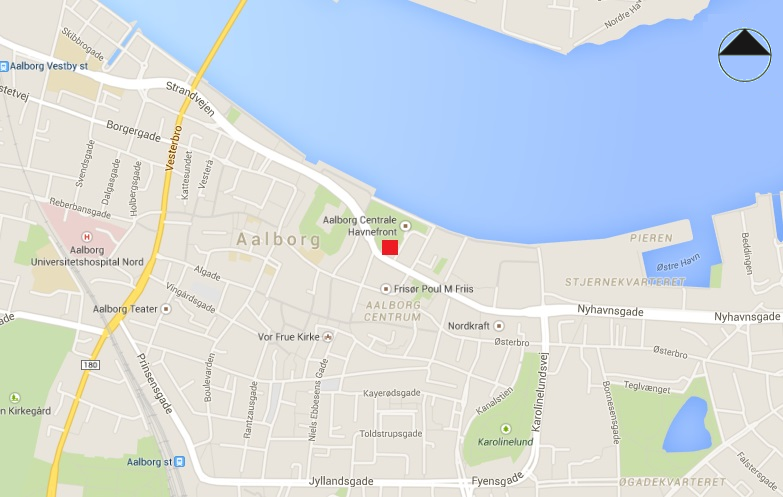
\includegraphics[width=1.0\textwidth]{billeder/aalborg.png}
	\caption{Strøybergs Palæs beliggenhed}
	\label{fig:aalborg}
\end{figure}

\indent{     }  Når der skal anlægges nye arealer, bygninger, veje osv., skal det opføres i henhold til en lokalplan, der dækker et mindre område inden for kommunen, og har til formål at styre udviklingen indenfor dette område ved hjælp af fastlagte regler og målsætninger. Den gældende lokalplan for området ved Strøybergs Palæ er lokalplan 1-1-107.
\newline
\newline
Ved en tilbygning til Strøybergs Palæ skal der tages højde for lokalplanen, men det er ikke alt. Der skal beregnes, hvilke laster som konstruktionen vil blive påvirket af, før det efterfølgende er muligt at bestemme, hvilken ståltype og stålprofil, der skal anvendes, for at konstruktionen opnår en tilstrækkelig bæreevne. Hertil skal brudgrænsetilstanden og anvendelsesgrænsetilstanden beregnes, da disse er dimensionsgivende for en konstruktion; brudgrænsetilstanden giver et mål for, om der opstår brud i konstruktionens stålrammer, eller om de har en tilstrækkelig styrke, mens anvendelsesgrænsetilstanden giver et mål for, hvor stor udbøjning stængerne oplever ved lasterne. 
\newline \indent{     }  Lasterne vil optræde som både permanente laster, hvor egen- og jordlasten regnes ud for tilbygningen, og som variable laster, der afhænger af anvendelsen af tilbygningen samt vejrforholdene.
\newline \indent{     }  For at bestemme bæreevnen gennem brudgrænsetilstanden opstilles først en række lastkombinationer for forskellige lasttilfælde, og derefter bestemmes reaktioner og snitkræfter for konstruktionen ud fra den lastkombination, som formodes at give de mest kritiske belastninger. 
\newline \indent{     }  For anvendelsesgrænsetilstanden skal udbøjningen bestemmes, da en tilstrækkelig bæreevne ikke altid er dimensionsgivende for en konstruktion. Der findes ikke nogle fastsatte normer for størrelsen af udbøjningen, men der er vejledende mål i Eurocode 1993 for, hvor stor udbøjning der tillades, før det føles sikkert at færdes i bygningen. De endelige mål fastsættes af bygherre.
\newline
\newline
De geologiske forhold for området omkring Strøybergs Palæ er også vigtige at kende til, før en tilbygning kan udføres, da konstruktionen skal bæres af jordlagene under bygningen. Derfor laves en udredning for geologien i Aalborg for at for at få en viden omkring, hvilken funderingstype, der er optimal at anvende til tilbygningen. I denne rapport ønskes en bestemt funderingstype; direkte fundering. Til bestemmelse af fundamentet ønskes friktionsvinklen bestemt, hvilket vil gøres ud fra fire forsøg, som vil blive beskrevet i rapporten.